\documentclass[usenames,dvipsnames,aspectratio=169]{beamer}

\usepackage[utf8]{inputenc}
\usepackage[T1]{fontenc}
\usepackage[magyar]{babel}
\usepackage{indentfirst}
\usepackage{graphicx}
\usepackage{listingsutf8}
\lstset{literate=
  {á}{{\'a}}1 {é}{{\'e}}1 {í}{{\'i}}1 {ó}{{\'o}}1 {ú}{{\'u}}1
  {Á}{{\'A}}1 {É}{{\'E}}1 {Í}{{\'I}}1 {Ó}{{\'O}}1 {Ú}{{\'U}}1
  {à}{{\`a}}1 {è}{{\`e}}1 {ì}{{\`i}}1 {ò}{{\`o}}1 {ù}{{\`u}}1
  {À}{{\`A}}1 {È}{{\'E}}1 {Ì}{{\`I}}1 {Ò}{{\`O}}1 {Ù}{{\`U}}1
  {ä}{{\"a}}1 {ë}{{\"e}}1 {ï}{{\"i}}1 {ö}{{\"o}}1 {ü}{{\"u}}1
  {Ä}{{\"A}}1 {Ë}{{\"E}}1 {Ï}{{\"I}}1 {Ö}{{\"O}}1 {Ü}{{\"U}}1
  {â}{{\^a}}1 {ê}{{\^e}}1 {î}{{\^i}}1 {ô}{{\^o}}1 {û}{{\^u}}1
  {Â}{{\^A}}1 {Ê}{{\^E}}1 {Î}{{\^I}}1 {Ô}{{\^O}}1 {Û}{{\^U}}1
  {œ}{{\oe}}1 {Œ}{{\OE}}1 {æ}{{\ae}}1 {Æ}{{\AE}}1 {ß}{{\ss}}1
  {ç}{{\c c}}1 {Ç}{{\c C}}1 {ø}{{\o}}1 {å}{{\r a}}1 {Å}{{\r A}}1
  {€}{{\EUR}}1 {£}{{\pounds}}1 {ő}{{\H{o}}}1 {ű}{{\H{u}}}1
}
\lstdefinestyle{HTML}{
  language=HTML,
  breaklines=true,
  postbreak=\mbox{\textcolor{red}{$\hookrightarrow$}\space},
  stringstyle=\ttfamily,
  inputencoding=utf8,
  morekeywords={header, time, nav, main, article, section, aside, role, 
    footer, details, open, summary, srcdoc}
}
\usepackage{hyperref}
\usepackage{attachfile}
\usepackage{multirow}
% Navigációs pöttyök hozzáadása subsection nélküli fejezetekhez
\usepackage{remreset}
\makeatletter
\@removefromreset{subsection}{section}
\makeatother
\setcounter{subsection}{1}
%%%%%
\attachfilesetup{color={1.0 0.6 0.0},author={HFM},description={Kattintson duplán a minta %
megtekintéséhez!},icon=Paperclip}
\definecolor{kiemelesszin}{rgb}{0.6,0.0,0.0}
\definecolor{kiemelesszinZ}{rgb}{0.0,0.6,0.0}
\definecolor{kiemelesszinN}{RGB}{196,127,0}
\definecolor{hivatkozasszin}{rgb}{0.0,0.0,0.75}
\newcommand{\kiemel}[1]{{\color{kiemelesszin}#1}}
\newcommand{\kiemelZ}[1]{{\color{kiemelesszinZ}#1}}
\newcommand{\kiemelN}[1]{{\color{kiemelesszinN}#1}}
\newcommand{\hiv}[1]{{\color{hivatkozasszin}#1}}
\frenchspacing
\usetheme[compress]{Berlin}

\title[Web technológiák - HTML]{Egyszerű HTML5 weboldalak készítése}
\subtitle{(GKxB\_INTM049)}
\author{Dr. Hatwágner F. Miklós}
\institute{Széchenyi István Egyetem, Győr}
\date{\hiv{\href{https://github.com/wajzy/GKxB\_INTM049.git}{https://github.com/wajzy/GKxB\_INTM049.git}}\\ \today}

\begin{document}

%1
\begin{frame}[plain]
  \titlepage
\end{frame}

\section{Jelölőnyelvek}

%2
\begin{frame}
  \begin{itemize}
    \item Cél: a nyers szöveg egyes részeit strukturálni, jelentésbeli többletet hozzáadni (pl. fejezetcím, bekezdés)
    \item Történeti előzmény: nyomdai előkészítés, kéziratok szerkesztése, gépi szedőrendszerek
    \item Példák jelölőnyelvekre: 
      \hiv{\href{http://man7.org/linux/man-pages/man7/roff.7.html}{roff}}, 
      \hiv{\href{https://www.latex-project.org/}{LaTeX}}, 
      \hiv{\href{https://en.wikipedia.org/wiki/Standard_Generalized_Markup_Language}{SGML}}
  \end{itemize}
\end{frame}

\subsection{roff}

%3
\begin{frame}
  \footnotesize
  \begin{description}[m]
    \item[RUNOFF] \hfill \\ nyers szövegből és parancsokból (.XX) álló fájlok $\to$ tördelt megjelenítés buta terminálokon (OS: Compatible Time Sharing System, CTSS, 1963)
    \item[runoff] \hfill \\ a RUNOFF bővített képességű portja \emph{IBM Selectric} terminálokhoz (OS: Multiplexed Information and Computing Service, multics, $\approx$'60-as évek vége)
    \item[roff] \hfill \\ a runoff továbbfejlesztése a Bell Telephone Labs-nál (1973) a PDP-11 géphez kapcsolt \emph{Graphic Systems CAT} (grafikus szedőegység) miatt. A roff család:
    \begin{description}[m]
      \item[troff] \hfill \\ typesetter roff a CAT-hez
      \item[nroff] \hfill \\ terminálokhoz és nyomtatókhoz
      \item[roff] \hfill \\ korlátozott képességű runoff utód, nem fejlesztették tovább
    \end{description}
    \item[groff] \hfill \\ GNU implementáció, máig fejlesztik $\to$ man oldalak
  \end{description}
\end{frame}

%4
\begin{frame}
  \begin{columns}[c]
    \column{0.5\textwidth}
      \tiny
      \begin{exampleblock}{\textattachfile{groff.1}{/usr/share/man/man1/groff.1.gz/groff.1}}
        \lstinputlisting[language=,breaklines=true,linerange={1-3},numbers=left,firstnumber=1]{groff.1}
        \lstinputlisting[language=,basicstyle=\ttfamily,breaklines=true,postbreak=\mbox{\textcolor{red}{$\hookrightarrow$}\space},linerange={75-85},numbers=left,firstnumber=75]{groff.1}
      \end{exampleblock}
    \column{0.5\textwidth}
      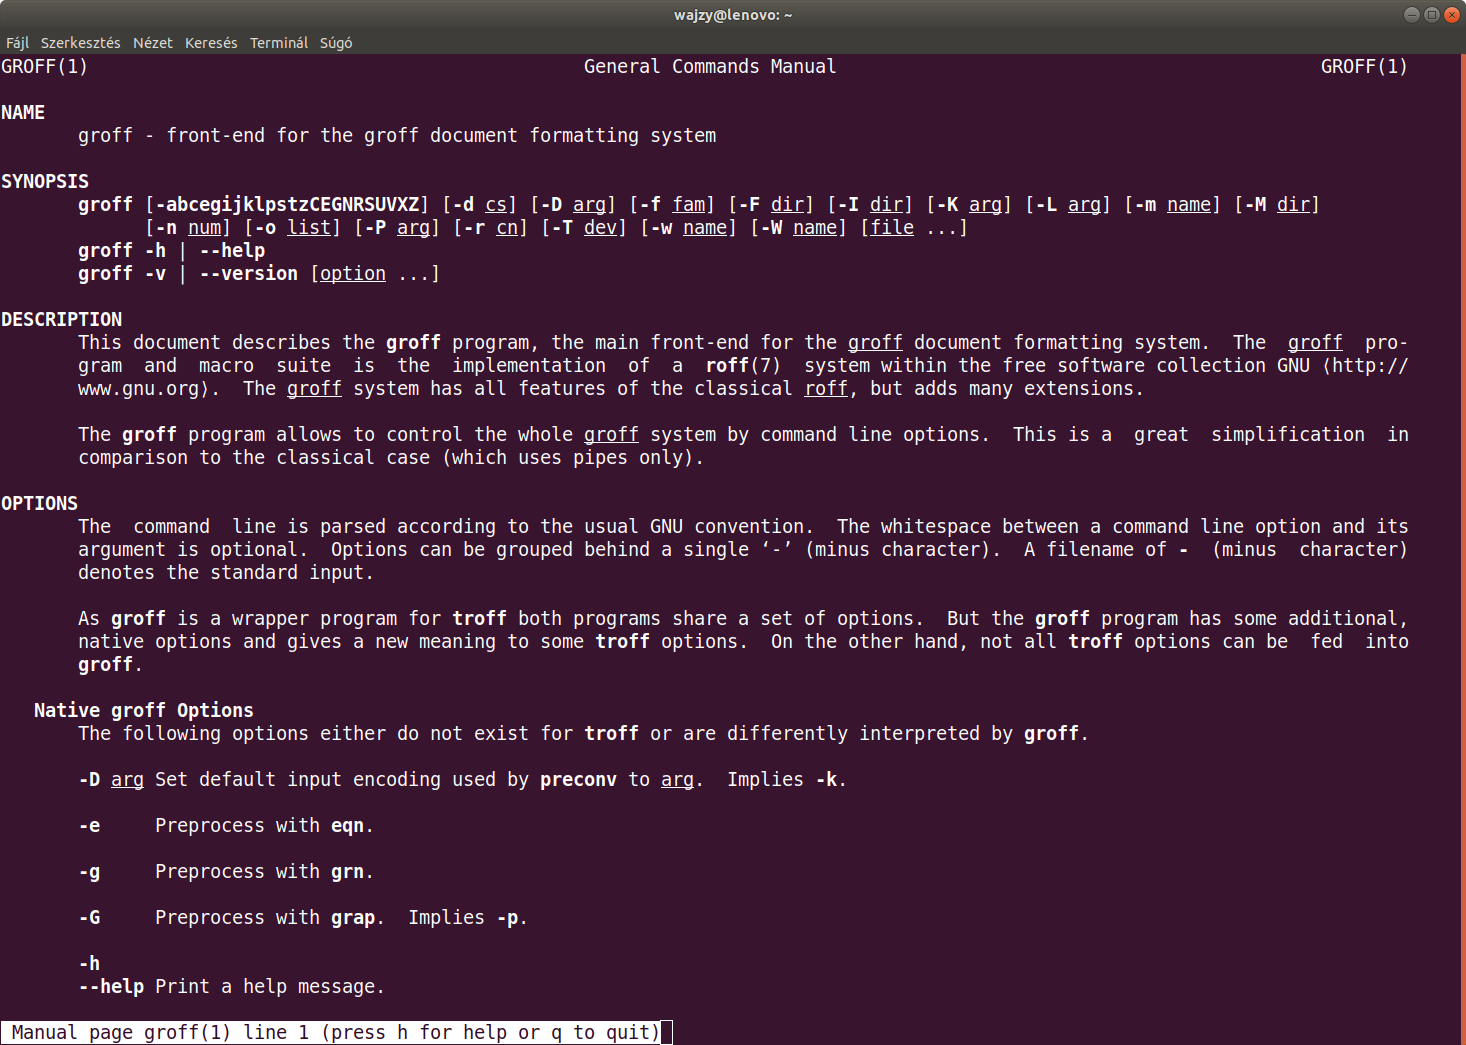
\includegraphics[width=\linewidth]{./groff.png}
  \end{columns}
\end{frame}

\subsection{\LaTeX{}}

%5
\begin{frame}
  \begin{columns}[T]
    \column{0.3\textwidth}
      \begin{description}[m]
        \item[\TeX] \hfill \\ Betűszedő rendszer, fejlesztője Donald E. Knuth, 1978 (Elégedetlenség \hiv{\href{https://www-cs-faculty.stanford.edu/~knuth/taocp.html}{könyvének}} szedésével.)
        \item[\LaTeX] \hfill \\ \TeX-en alapuló szövegformázó rendszer, Leslie Lamport, 1983
      \end{description}
    \column{0.7\textwidth}
        \begin{exampleblock}{\textattachfile{html.tex}{html.tex}}
          \centering
          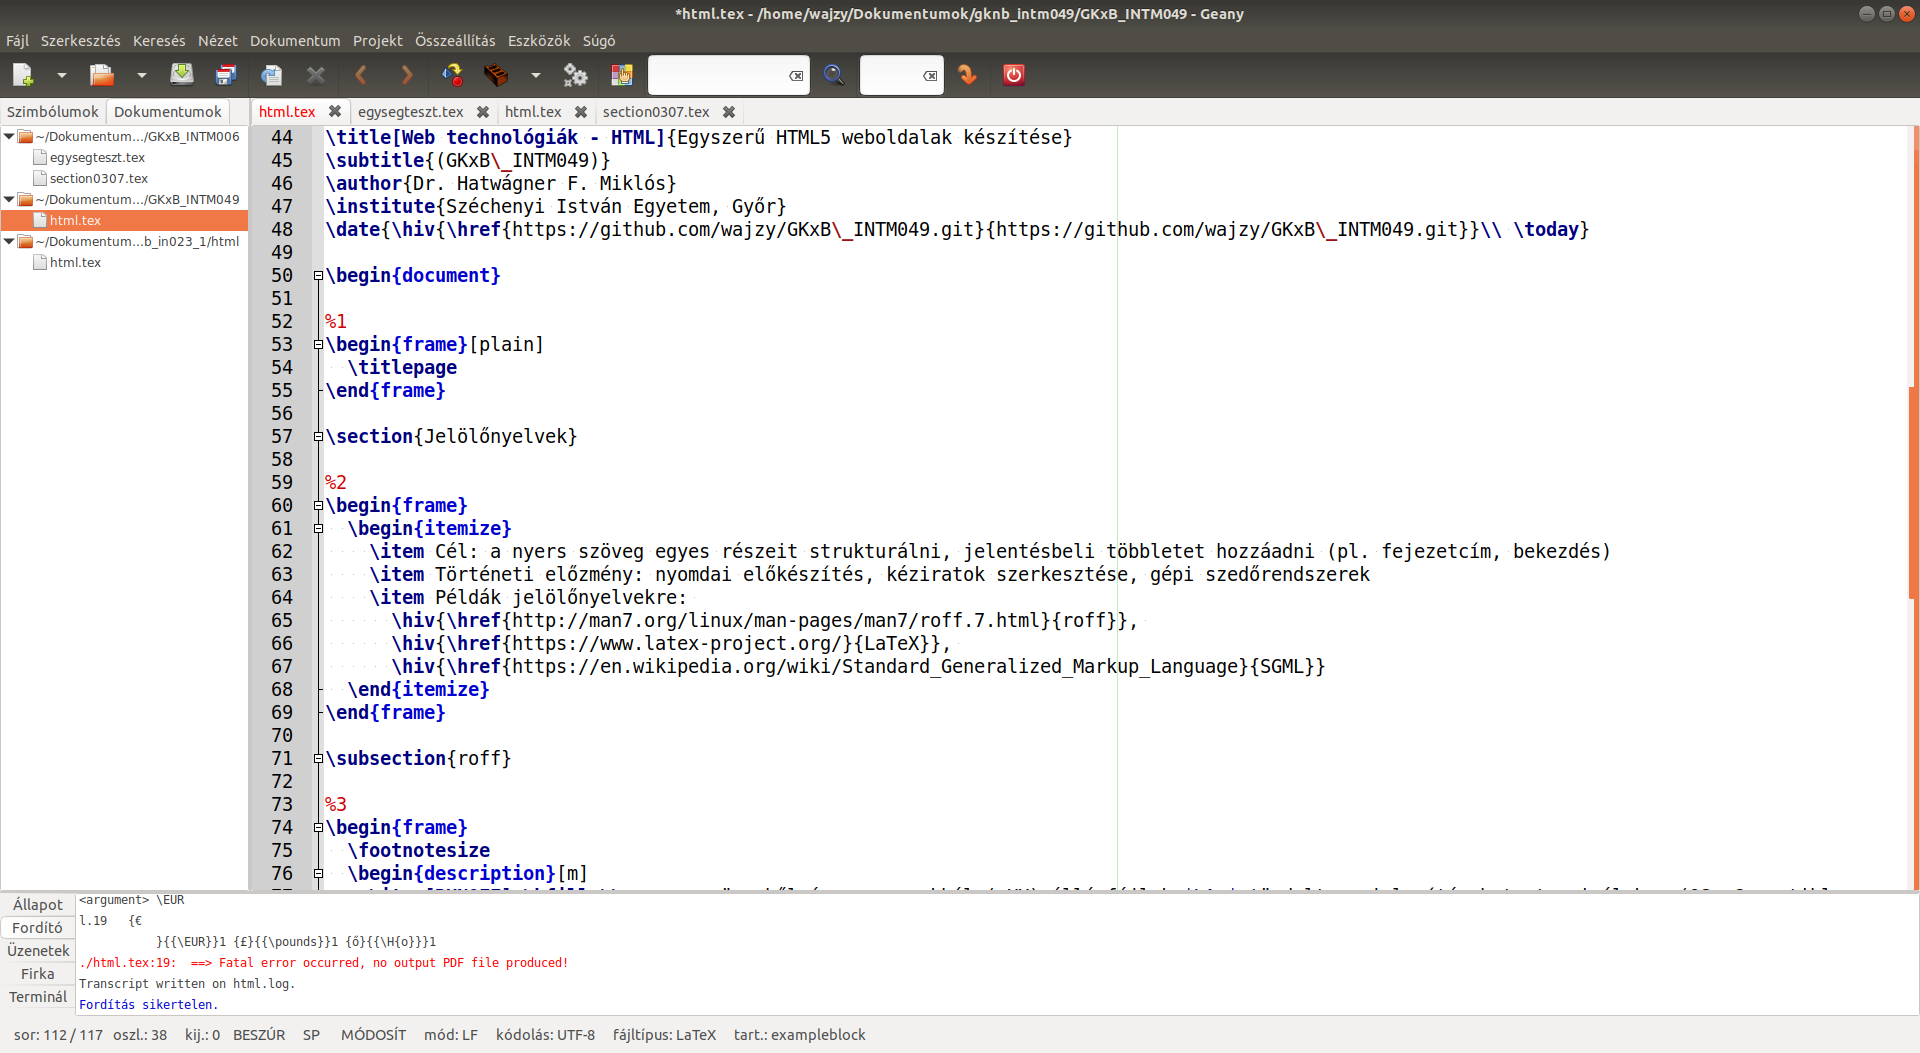
\includegraphics[scale=.14]{./latex.png}
        \end{exampleblock}
  \end{columns}
\end{frame}

\subsection{SGML}

%6
\begin{frame}
  \begin{itemize}
    \item SGML (Standard Generalized Markup Language), ISO 8879:1986
    \item Szabványos jelölőnyelv dokumentumok szerkezetének leírására,
beleértve a címkék definiálását is
    \item Gépfüggetlen metanyelv
    \item Előzménye: GML (1969)
    \begin{itemize}
      \item C. \kiemel{G}oldfarb (IBM), E. \kiemel{M}osher, R. \kiemel{L}orie
      \item dokumentumtípusonként egyedi kódolási séma definiálható
      \item előre definiált elemek egymásba ágyazhatóak
      \item először az IBM nyomdarendszere használta
    \end{itemize}
    \item Tulajdonságai
    \begin{itemize}
      \item Deklaratív: struktúrát és attribútumokat rögzít, nem a feldolgozás módját ($\to$~időtállóság)
      \item Gépi feldolgozás lehetősége
    \end{itemize}
  \end{itemize}
\end{frame}

%7
\begin{frame}
  \begin{itemize}
    \item Legfontosabb építőelemek
    \begin{itemize}
      \item Elemek ([element] nyitó és záró cimkék [tag] által határolva)
      \item A nyitó tagben attribútumok (kulcs-érték párok) adhatók meg
      \item Elemek egymásba ágyazhatóak
      \item Elemek, attribútumok alkalmazási szabályai $\to$ Document Type Definition (DTD)
    \end{itemize}
    \item Néhány korai, jelentős alkalmazás
    \begin{itemize}
      \item Electronic Manuscript Project of the Association of American Publishers (AAP, tudományos dokumentumok)
      \item Computer-aided Acquisition and Logistic Support (CALS, katonai dokumentumok kezelése)
      \item LinuxDoc (Linux csomagok)
    \end{itemize}
  \end{itemize}
\end{frame}

%8
\begin{frame}[fragile]
  \scriptsize
  \begin{columns}[T]
    \column{0.4\textwidth}
    \begin{exampleblock}{SGML példa}
      \begin{verbatim}
<!DOCTYPE PEOPLE SYSTEM 
  "people.dtd">
<PEOPLE DATE="15 6 2000">
 <NAME TITLE="Mr">
  <FIRST>Wally</FIRST>
  <LAST>Wallpaper</LAST>
 </NAME>
 <NAME>
  <LAST>Jackson</LAST>
 </NAME>
 <NAME TITLE="Dr">
  <FIRST>Susan</FIRST>
  <MIDDLE>Ramsay</MIDDLE>
  <LAST>Sukie</LAST>
 </NAME>
</PEOPLE>
\end{verbatim}
    \end{exampleblock}
    \column{0.6\textwidth}
    \begin{exampleblock}{people.dtd}
      \begin{verbatim}
<!ELEMENT people - - (name+)>
<!ATTLIST people date NUMBERS #REQUIRED>

<!ELEMENT name - - (first?, middle?, last)>
<!ATTLIST name title CDATA #IMPLIED>

<!ELEMENT first - - (#PCDATA)>
<!ELEMENT middle - - (#PCDATA)>
<!ELEMENT last - - (#PCDATA)>
\end{verbatim}
    \end{exampleblock}
    \tiny
    Forrás: \textattachfile{chap4.html}{OmniMark dokumentáció}
  \end{columns}
\end{frame}

\subsection{A HTML története}

%9
\begin{frame}
  \begin{itemize}
    \item ENQUIRE: a CERN dokumentumtároló, -megosztó szoftvere. (Tim Berners-Lee, 1980)
    \item HTML első említése: T.B.L., 1991 (18 elem, melyek a CERN SGMLguid-on, a kutatóintézet SGML alkalmazásán alapultak)
    \item A HTML egy SGML alkalmazás: 1993-2014
    \item HTML 4.01: Strict/Transitional/Frameset DTD, 1999
    \item Aktuális változat: \hiv{\href{https://www.w3.org/TR/html52/}{HTML5}}
    \item Néhány újdonság: videó- és hanglejátszás, vektorgrafika, többszálúsítás, helyi adattárolás, bittérképes grafika, stb.
    \item ,,Élő szabvány'', meghatározó szervezetek: \hiv{\href{https://www.w3.org/}{W3C}} (ajánlások), \hiv{\href{https://whatwg.org/}{WHATWG}} (innovatív technológiák)
    \item 2019-től a WHATWG tartja karban a HTML szabványát.
    \item XHTML: XML előírásoknak megfelelő HTML; a HTML5 ,,feleslegessé'' tette
  \end{itemize}
\end{frame}


\section{HTML5}

\subsection{Általános tulajdonságok}

\subsection{Általános tulajdonságok}

%10
\begin{frame}
  \begin{itemize}
    \item Egyszerű szövegfájl (jellemzően UTF-8 kódolással)
    \item Dokumentum \emph{strukturájának} jelölésére, pl.
    \begin{itemize}
      \item fejlécek
      \item listák
      \item bekezdések
      \item hiperhivatkozások
    \end{itemize}
    \item Megjelenítést befolyásolja
    \begin{itemize}
      \item böngésző alapértelmezése
      \item felhasználó globális beállításai a böngészőben
      \item stíluslapok (CSS)
    \end{itemize}
    \item Megjelenítés leválasztása
    \begin{itemize}
      \item helyes megjelenítés többféle böngészőben
      \item könnyebben karbantartható oldalak
      \item nem vizuális böngészők támogatása
    \end{itemize}
  \end{itemize}
\end{frame}

%11
\begin{frame}
  \begin{itemize}
    \item Struktúra kialakítása az SGML-hez hasonlóan: egymásba ágyazható elemek, címkék, attribútumok
    \item Beágyazási szabályok, használható attribútumok $\to$ ,,szabvány'' (ajánlás)
    \item Helytelenül formázott dokumentumok
    \begin{itemize}
      \item Nincsenek hibaüzenetek
      \item A böngésző a tőle telhető legjobb eredményt nyújtja
      \item Kompatibilitási okokból az elavult megoldásokat is kénytelen támogatni
      \item Ellenőrzés különböző böngészőkben vs. \hiv{\href{https://validator.w3.org/}{szintaxis validálás}}
    \end{itemize}
  \end{itemize}
\end{frame}

%12
\begin{frame}
  \scriptsize
  \begin{exampleblock}{\textattachfile{hibas.html}{hibas.html}}
    \lstinputlisting[language=HTML]{hibas.html}
  \end{exampleblock}
  \begin{columns}[T]
    \column{0.3\textwidth}
      \begin{center}
        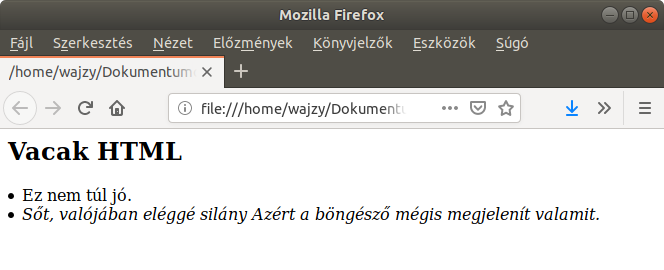
\includegraphics[width=\textwidth]{hibas_firefox.png} \\
        Mozilla Firefox 69.0
      \end{center}
    \column{0.3\textwidth}
      \begin{center}
        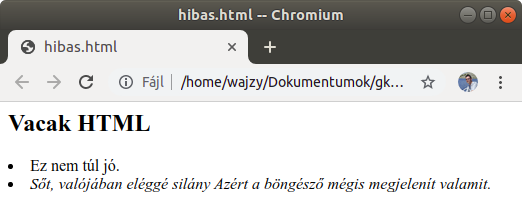
\includegraphics[width=\textwidth]{hibas_chromium.png} \\
        Chromium 76.0.3809.100
      \end{center}
    \column{0.3\textwidth}
      \begin{center}
        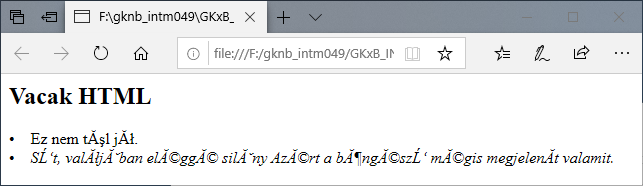
\includegraphics[width=\textwidth]{hibas_edge.png} \\
        Microsoft Edge 44.17763.1.0
      \end{center}
  \end{columns}
\end{frame}


\subsection{Az első HTML oldal elkészítése}

\subsection{Az első HTML oldal elkészítése}

%13
\begin{frame}
  Válasszunk egy szövegszerkesztőt (pl. 
    \hiv{\href{https://www.geany.org/}{Geany}}, 
    \hiv{\href{https://code.visualstudio.com/}{VS Code}}, 
    \hiv{\href{https://notepad-plus-plus.org/}{NotePad++}}, \dots), 
    gépeljük be és mentsük ki az alábbi fájlt \texttt{elso.html} néven, UTF-8 kódolással!
    \footnotesize
    \begin{exampleblock}{\textattachfile{elso.html}{elso.html}}
      \lstinputlisting[style=HTML]{elso.html}
    \end{exampleblock}
\end{frame}

%14
\begin{frame}
  Dokumentum típusának meghatározása
  \begin{description}[m]
    \item[HTML5] \kiemel{Nincs DTD!} \hfill \\
      <!DOCTYPE html>
    \item[4.01, Szigorú] \hfill \\
      <!DOCTYPE HTML PUBLIC "-//W3C//DTD HTML 4.01//EN" "http://www.w3.org/TR/html4/strict.dtd">
    \item[4.01, Átmeneti] \hfill \\
      <!DOCTYPE HTML PUBLIC "-//W3C//DTD HTML 4.01 Transitional//EN" "http://www.w3.org/TR/html4/loose.dtd">
    \item[4.01, Keretek] \hfill \\
      <!DOCTYPE HTML PUBLIC "-//W3C//DTD HTML 4.01 Frameset//EN" "http://www.w3.org/TR/html4/frameset.dtd">
    \end{description}
\end{frame}

%15
\begin{frame}
  Elemek (element)
  \begin{itemize}
    \item Általában nyitó és záró cimkék (tag) között, pl. \texttt{<body>\dots</body>}, \texttt{<p>\dots</p>}
    \item Néha a böngésző kitalálja, hol kellene lennie az elem (pl. \texttt{<p>}, \texttt{<li>}) záró címkéjének, így az elhagyható, de \kiemel{nem javasolt} (XML elemző számára szabálytalanná teszi a fájlt)
    \item Léteznek üres elemek is; itt nincs mit közbezárni címkékkel, pl. \texttt{<meta />}, vízszintes vonal \texttt{<hr~/>} vagy \texttt{<hr>}
    \item Rögzített szabályok szerint egymásba ágyazhatók
    \item Kis- és nagybetűkre érzéketlen, de \kiemel{ajánlott} a kisbetűs írásmód
    \item A szöveg tördelése független a forrásszöveg tördelésétől (pl. az egymás mellé gépelt fehér karaktereket egynek tekinti)
    \item Címkék mindig \kiemel{<} és \kiemel{>} jelek között
    \item Jelentéssel bíró karakterek bevitele \hiv{\href{https://en.wikipedia.org/wiki/List_of_XML_and_HTML_character_entity_references\#Character_entity_references_in_HTML}{entitásokkal}} (pl. \kiemel{<} $\to$ \kiemel{\&lt;} vagy \kiemel{>} $\to$ \kiemel{\&gt;})
  \end{itemize}
\end{frame}

%16
\begin{frame}
  Elemek
  \begin{description}[m]
    \item[\texttt{<html>}] gyökérelem, pontosan egynek kell lennie (dokumentum nyelve attribútummal, ld. )
    \item[\texttt{<head>}] metaadatok
    \begin{description}
      \item[\texttt{<title>}] dokumentum címe (böngészőablak vagy -fül felirata)
      \item[\texttt{<meta>}] általános metaadat
    \end{description}
    \item[\texttt{<body>}] megjelenítendő tartalom
    \begin{description}
      \item[\texttt{<h1>}] ,,Címsor1''
      \item[\texttt{<p>}] Bekezdés (paragraph)
    \end{description}
  \end{description}
  \vfill
  Megjegyzések\\
  \kiemel{\texttt{<!{-}-}} és \kiemel{\texttt{{-}->}} között 
\end{frame}

%17
\begin{frame}
  Attribútumok
  \begin{itemize}
    \item Mindig a nyitó címkében (pl. \texttt{<html lang="hu-HU">}, \hiv{\href{http://www.ietf.org/rfc/rfc1766.txt}{RFC1766}} szerint)
    \item Kulcs-érték párok, = jellel elválasztva
    \item \kiemel{Ajánlott} a kulcsot kisbetűvel írni
    \item Az értéket \kiemel{ajánlott} idézni, lehetőleg ''-vel (de az ' is megfelel; szóközt tartalmazó értéknél pedig kötelező)
    \item Egy címkében lehet több attribútum is
    \item Vagy egy sem (minimalizált szintaxis); itt az attribútum léte hordoz információt (pl. \texttt{<p hidden>}). XML feldolgozók megkövetelik az értéket, pl. \texttt{<p~hidden="hidden">}
  \end{itemize}
\end{frame}


\subsection{Címsorok}

\subsection{Címsorok}

%18
\begin{frame}
  \begin{itemize}
    \item \texttt{<h1>}, \texttt{<h2>}, \dots, \texttt{<h6>}: legmagasabbtól legalacsonyabb szintig
    \item Például: \texttt{<h1>Első fejezet, amelyben bemutatnak bennünket Micimackónak és a méheknek, mellékesen a könyv is elkezdődik</h1>}
    \item Általában nagyobb betűméretek és a címsor elé és/vagy mögé tett térközök jellemzik
    \item Keresőmotorok is használhatják a dokumentum struktúrájának feltérképezésére
    \item Tematikus részek elválasztására gyakran elválasztó vonalat (\texttt{<hr />}) használnak
  \end{itemize}
\end{frame}

%19
\begin{frame}
  \begin{columns}[c]
    \column{0.5\textwidth}
      Készítsen weboldalt, ami egymás alá írja a \emph{Címsor1}, \emph{Címsor2}, \dots, \emph{Címsor6} szövegeket, a nekik megfelelő HTML elemekkel, a 3. és a 4. szövegsor között pedig húz egy vízszintes vonalat!
    \column{0.5\textwidth}
      \begin{exampleblock}{\textattachfile{cimsorok.html}{cimsorok.html}}
        \begin{center}
          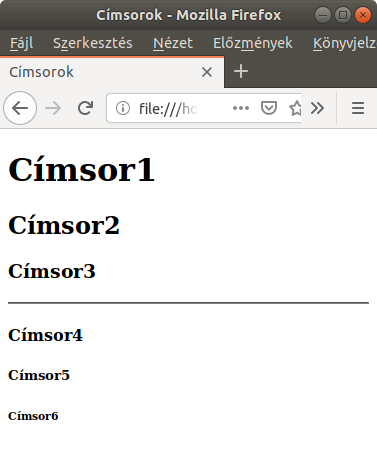
\includegraphics[scale=.25]{cimsorok.png}
        \end{center}
      \end{exampleblock}
  \end{columns}
\end{frame}


\subsection{Bekezdések}

\subsection{Bekezdések}

%20
\begin{frame}
  \small
  \begin{itemize}
    \item Bekezdések \texttt{<p>} elemmel jelölhetők
    \item Például: \texttt{<p title="Bek. 1">Első bekezdés.</p><p>Második bekezdés.</p>}
    \item Alapértelmezetten térközt hagy a böngésző a bekezdések között
    \item Sortörés új bekezdés (és térköz) nélkül: \texttt{<br />}
    \item Előformázott szöveg (pl. karakteres módú program kimenete), egyenszélességű (monospace) karakterekkel, forrás fehér karaktereinek megőrzésével: \texttt{<pre>}
  \end{itemize}
  \vfill
  ,,Tradicionális'' \hiv{\href{https://developer.mozilla.org/en-US/docs/Web/HTML/Block-level_elements}{tördelési módok}}
  \begin{description}[m]
    \item[Blokkszintű] (block) \hfill \\ Új sorban kezdődik, és a teljes elérhető szélességet elhasználja, pl. \texttt{<p>}, \texttt{<pre>}, \texttt{<h1>}-\texttt{<h6>}, \texttt{<hr />}
    \item[Soron belüli] (inline) \hfill \\ Aktuális sorban kezdődik, csak olyan széles helyet foglal, ahol éppen elfér, pl. \texttt{<br />}
  \end{description}
\end{frame}

%21
\begin{frame}
  \begin{columns}[c]
    \column{0.75\textwidth}
      Formázza meg a \textattachfile{attila.txt}{verset} a mellékelt ábra szerint, azaz
      \begin{itemize}
        \item a költő neve legyen első szintű címsor, 
        \item a mű címe második szintű,
        \item a szakaszok (arab számokkal jelölve) harmadik szintűek.
        \item A bekezdéseket és a bekezdésen belüli sortöreseket állítsa be!
        \item A bekezdések fölé mozgatva az egeret lássuk a bekezdés sorszámát, pl. 1/1, 1/2, \dots, 2/3
      \end{itemize}
    \column{0.25\textwidth}
      \begin{center}
        \begin{exampleblock}{\textattachfile{attila.html}{attila.html}}
          \centering 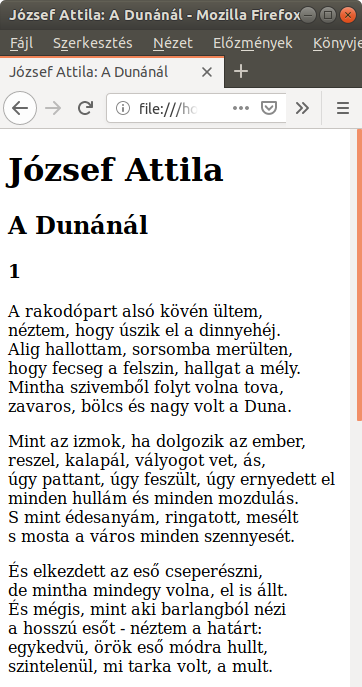
\includegraphics[scale=.2]{attila.png}
        \end{exampleblock}
      \end{center}
  \end{columns}
\end{frame}

%22
\begin{frame}
  \begin{columns}[c]
    \column{0.7\textwidth}
      Formázza meg a klasszikus Fahrenheit-Celsius átváltó 
      \textattachfile{fahrcels.c}{program} \textattachfile{fahrcels.txt}{kimenetét} 
      a mellékelt ábra szerint, azaz őrizze meg a program karakteres kimenetének formázását 
      a \texttt{<pre>} elemmel!
      
      A \texttt{<pre>} elem megőrzi a HTML forrásban lévő szóközöket, sortöréseket, és monospace betűtípust használ.
    \column{0.3\textwidth}
      \begin{center}
        \begin{exampleblock}{\textattachfile{fahrcels.html}{fahrcels.html}}
          \centering 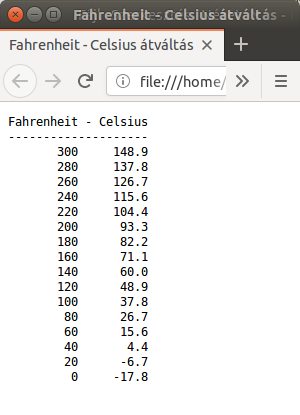
\includegraphics[scale=.35]{fahrcels.png}
        \end{exampleblock}
      \end{center}
  \end{columns}
\end{frame}


\subsection{Soron belüli jelölések}

\subsection{Soron belüli jelölések}

%23
\begin{frame}
  A soron belüli formázó elemek közül előnyben részesítjük azok használatát, melyek \emph{szemantikai többletet}
  adnak a szöveg tartalmának, a pusztán \emph{formázási célú} elemekkel szemben $\to$ erre ott a CSS!
  \vfill
  Ettől függetlenül, néhány, csak formázási célú elem használata továbbra is szabványos a HTML5-ben.
  \vfill
  \begin{description}[m]
    \item[\texttt{<small>}] \hfill \\ Kisbetűs szöveg. (A \texttt{<big>} elem a HTML5-ben már nem támogatott.)
    \item[\texttt{<i>}] (italics) \hfill \\ Döntötten szedett szöveg, jelentéstöbblet nélkül.
    \item[\texttt{<em>}] (emphasized) \hfill \\ Hangsúlyos, fontos szövegrész, melyet a böngésző alapértelmezetten általában dőlt betűkkel jelenít meg.
  \end{description}
\end{frame}

%24
\begin{frame}
  \begin{description}[m]
    \small
    \item[\texttt{<b>}] (bold) \hfill \\ Félkövéren szedett szöveg, jelentéstöbblet nélkül.
    \item[\texttt{<strong>}] (strong importance) \hfill \\ Kiemelten hangsúlyos, fontos szövegrész, melyet a böngésző alapértelmezetten általában félkövér betűkkel jelenít meg.
    \item[\texttt{<sup>}] (superscript) \hfill \\ Felső index.
    \item[\texttt{<sub>}] (subscript) \hfill \\ Alsó index.
    \item[\texttt{<ins>}] (inserted) \hfill \\ Utólag beszúrt szöveg (ált. aláhúzással jelölve).
    \item[\texttt{<del>}] (deleted) \hfill \\ Kitörölt szöveg (ált. áthúzással jelölve).
    \item[\texttt{<mark>}] \hfill \\ Kijelölt szöveg (ált. sárga háttérrel kiemelve).
  \end{description}
\end{frame}

%25
\begin{frame}
  \begin{columns}[c]
    \column{0.7\textwidth}
      Próbálja meg előállítani azt a HTML fájlt, ami a jobb oldalon látható módon jelenik meg a böngészőben!
      Kiinduláshoz felhasználhatja a dokumentum \textattachfile{soronbelul.txt}{nyers szövegét}.
      Ne feledje, hogy az olyan, önmagukban is jelentéssel bíró karakterek megjelenítése, mint pl. a \kiemel{<}
      karakter, \hiv{\href{https://en.wikipedia.org/wiki/List_of_XML_and_HTML_character_entity_references\#Character_entity_references_in_HTML}{HTML entitásokkal}} lehetséges.
    \column{0.3\textwidth}
      \begin{center}
        \begin{exampleblock}{\textattachfile{soronbelul.html}{soronbelul.html}}
          \centering 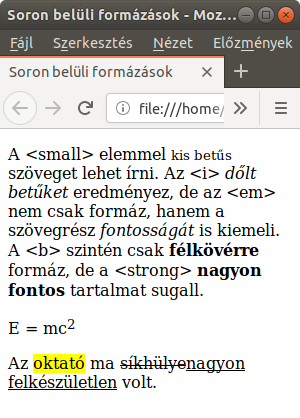
\includegraphics[scale=.35]{soronbelul.png}
        \end{exampleblock}
      \end{center}
  \end{columns}
\end{frame}


\subsection{Idézés, címek, írásirány}

\subsection{Idézés, címek, írásirány}

%26
\begin{frame}
  Szövegrészek idézése. Forrás jelölése: \texttt{cite} attribútummal.
  \begin{description}[m]
    \item[\texttt{<q>}] (quote) \hfill \\ Rövid szövegrészlet idézése, ált. automatikusan körbeveszi a böngésző idézőjelekkel. Soron belüli elem.
    \item[\texttt{<blockquote>}] \hfill \\ Hosszú szövegrészek, bekezdések idézése. Jellemzően behúzással formázva. Blokkszintű elem.
  \end{description}
  \vfill
  Rövidítések. Kifejtés megadható: \texttt{title} globális attribútummal.
  \begin{description}[m]
    \item[\texttt{<abbr>}] \hfill \\ Rövidítések és betűszavak jelöléséhez. Soron belüli elem.
    \item[\texttt{<acronym>}] \hfill \\ Betűszavak jelöléséhez használták, \kiemel{ELAVULT}.
  \end{description}
\end{frame}

%27
\begin{frame}
  Szöveg írásirányának jelölése: \texttt{dir} globális attribútummal, alapértelmezést a nyelvvel együtt a \texttt{html} elemben kell állítani. Értékek:
  \begin{description}[m]
    \item[\texttt{ltr}] (left to right) \hfill \\ balról jobbra
    \item[\texttt{rtl}] (right to left) \hfill \\ jobbról balra
  \end{description}
  \vfill
  Írásirány helyi módosítása: \texttt{<bdo>} (Bi-Directional Override) elemmel, \texttt{dir} attribútummal
  \vfill
  Mű címének jelölése: \texttt{<cite>} soron belüli elemmel.
  \vfill
  Postacím megadása: \texttt{<address>} blokkszintű elemmel.
\end{frame}

%28
\begin{frame}
  \begin{columns}[c]
    \column{0.6\textwidth}
      Próbálja meg előállítani azt a HTML fájlt, ami a jobb oldalon látható módon jelenik meg a böngészőben!
      Kiinduláshoz felhasználhatja a dokumentum \textattachfile{idezes.txt}{nyers szövegét}.
      A gondolatjelek többféle szélességben elérhetők: \texttt{\&ndash;}, \texttt{\&mdash;}.
    \column{0.4\textwidth}
      \begin{center}
        \begin{exampleblock}{\textattachfile{idezes.html}{idezes.html}}
          \centering 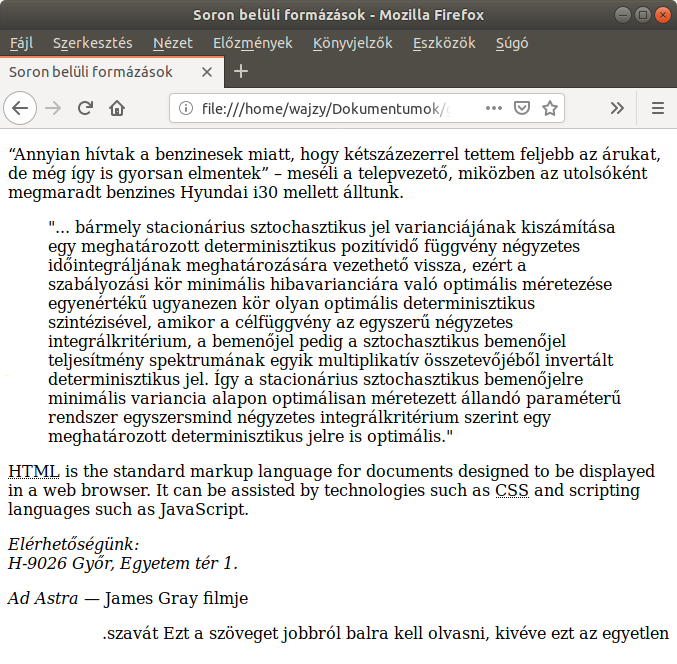
\includegraphics[scale=.23]{idezes.png}
        \end{exampleblock}
      \end{center}
  \end{columns}
\end{frame}


\subsection{Képek és hivatkozások}

\subsection{Képek és hivatkozások}

%29
\begin{frame}
  Képeket az \texttt{<img>} üres, soron belüli elemmel adunk meg. Attribútumok:
  \begin{description}[m]
    \item[\texttt{alt}] (alternate text) \hfill \\ Kép leírása (gyengénlátók, szöveges böngészők, stb. számára), kötelező.
    \item[\texttt{src}] (source) \hfill \\ Teljes/relatív elérési útvonal, URL
    \item[\texttt{width}] \hfill \\ Szélesség képpontokban
    \item[\texttt{height}] \hfill \\ Magasság képpontokban
  \end{description}
  Bár a méretet megadó attribútumok nem elavultak, \emph{ajánlott} a méretet CSS-sel megadni (CSS szabályok felülbírálják az attribútumok tartalmát). Az oldalak felesleges újratördelése elkerülhető a méretek megadásával.
\end{frame}

%30
\begin{frame}[fragile]
  Széles körben támogatott formátumok: jpeg, gif, png.
  \vfill
  Képek (\texttt{<img>} elemek) beágyazhatók a \texttt{<figure>} blokk szintű elembe.\\
  Célszerű beágyazni a kép feliratát is \texttt{<figcaption>} elemben.
  \vfill
  Például:
  \begin{verbatim}
<figure>
  <img alt="kep" src="kep.jpeg" width="320" height="240 /">
  <figcaption>Az egyetem logoja</figcaption>
</figure>
  \end{verbatim}
\end{frame}

%31
\begin{frame}
  \begin{columns}[c]
    \column{0.85\textwidth}
      Készítse el az alábbi oldalt! Képek adatai:
      \begin{enumerate}
        \item Forrás: \textattachfile{SZElogo.png}{SZElogo.png}, méret: 7088x2363 (kicsinyítse 10\%-ra!)
        \item Forrás: \textattachfile{html.gif}{html.gif}, méret: 500x400
        \item Forrás: \hiv{\href{https://www.w3.org/html/logo/downloads/HTML5\_Logo\_256.png}{https://www.w3.org/html/logo/downloads/HTML5\_Logo\_256.png}}, méret: 256x256
      \end{enumerate}
    \column{0.15\textwidth}
        \begin{center}
          \begin{exampleblock}{\textattachfile{kep.html}{kep.html}}
            \centering 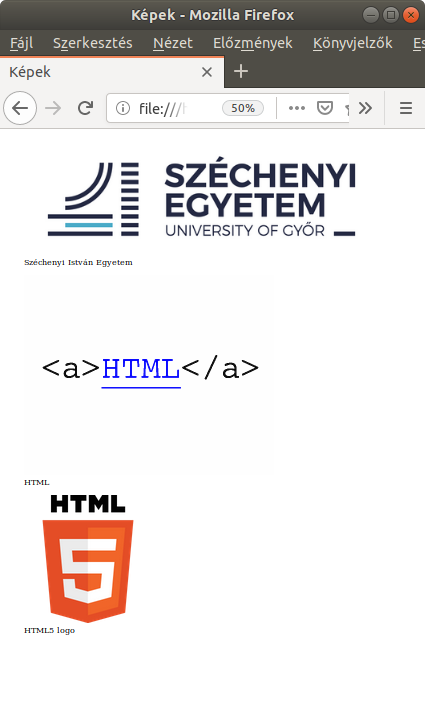
\includegraphics[scale=.14]{kep.png}
          \end{exampleblock}
        \end{center}
  \end{columns}  
\end{frame}

%_
\begin{frame}
  Néha a képfájlokat nem tudjuk/akarjuk feltölteni egy szerverre $\to$ beágyazzuk őket a weboldalba \hiv{\href{https://tools.ietf.org/html/rfc2397}{Data URL}}-ek segítségével:
  \vfill
  \begin{exampleblock}{Általános felépítés}
    \texttt{data:[<mediatype>][;base64],<data>}
  \end{exampleblock}
  \begin{exampleblock}{\textattachfile{dataurl.html}{dataurl.html}}
    \scriptsize
    \texttt{<img src="data:image/svg+xml;base64,PD94bWwgdmV...ZnPg0K" alt="IT logo" width="25\%" />}
  \end{exampleblock}
  \vfill
  \small
  \begin{itemize}
    \item Nem csak képek forrása adható meg ilyen módon, de ez a leginkább jellemző.
    \item Sok böngészőnél az URL hossza nem haladhatja meg a 64kB-ot.
    \item Base64 kódolást lehet végezni Linuxon/Max OS-en a \hiv{\href{https://linux.die.net/man/1/base64}{base64}} programmal, de vannak \hiv{\href{https://www.base64-image.de/}{online}} \hiv{\href{https://www.base64encode.org/}{eszközök}} is.
  \end{itemize}
\end{frame}

%32
\begin{frame}
  Kis kijelzőre nincs értelme túl nagy képet letölteni, majd összezsugorítani $\to$ eszközfüggő képek letöltése \emph{CSS3 media query} segítségével
  \begin{columns}
    \column{0.7\textwidth}
      \begin{exampleblock}{\textattachfile{kepmeret.html}{kepmeret.html}}
        \tiny
        \lstinputlisting[style=HTML,linerange={8-15},numbers=left,firstnumber=8]{kepmeret.html}
      \end{exampleblock}
    \column{0.3\textwidth}
      \centering 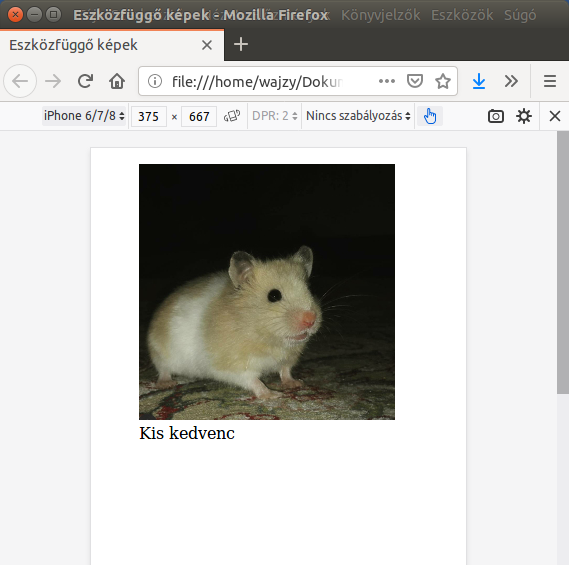
\includegraphics[scale=.18]{kepmeret.png}
  \end{columns} 
  \begin{enumerate}
    \item A böngésző az első, feltételeknek megfelelő képet fogja használni.
    \item Az utolsó beágyazott elem egy \texttt{<img>} legyen! (Kompatibilitás miatt, és alapértelmezett képet is definiál.)
  \end{enumerate}
\end{frame}

%33
\begin{frame}
  \footnotesize
  Hiperhivatkozások készíthetők \texttt{<a>} (anchor) soron belüli elemmel. A nyitó és záró címkék közötti szöveg/kép az érzékeny terület. Attribútumok:
  \begin{description}[m]
    \item[\texttt{href}] (hypertext reference) \hfill \\ Abszolút/relatív útvonal/URL, az ugrás célja. Könyvtár megadás esetén célszerű / jellel zárni.
    \item[\texttt{target}] \hfill \\ Hol nyíljon meg a betöltött tartalom? Értéke lehet:
    \begin{itemize}
      \item \texttt{\_blank} Új ablakban/fülön
      \item \texttt{\_self} Ugyanott, ahol a link is található (alapértelmezés)
      \item \texttt{\_parent} Szülő keretben. (A keretek \kiemel{ELAVULTAK}.)
      \item \texttt{\_top} A teljes ablakban, a keretből ,,kitörve''. (A keretek \kiemel{ELAVULTAK}.)
      \item \emph{keretnév} Adott nevű keretben. (A keretek \kiemel{ELAVULTAK}.)
    \end{itemize}
    \item[\texttt{title}] \hfill \\ Tooltip szöveg
  \end{description}
  Például: \texttt{<a href="https://www.google.com/">Ugrás a kereső oldalára</a>}
\end{frame}

%34
\begin{frame}
  \begin{columns}[c]
    \column{0.5\textwidth}
      Az ábrának megfelelően készítsen három hivatkozást egymás alatti bekezdésekben!
      \begin{itemize}
        \item A Széchenyi Egyetem oldalát az aktuális oldal helyére kell betölteni,
        \item az Edutusét új ablakba/fülre! 
        \item Végül a \textattachfile{HTML5sticker.png}{HTML5sticker.png} képet használva lehessen eljutni a W3C oldalára!
      \end{itemize}
      Készítsen feliratokat (SZE, Edutus, HTML5), melyek megjelennek az egeret a link fölé mozgatva!
    \column{0.5\textwidth}
      \begin{center}
        \begin{exampleblock}{\textattachfile{hivatkozas.html}{hivatkozas.html}}
          \centering 
\includegraphics[scale=.2]{hivatkozas.png}
        \end{exampleblock}
      \end{center}
  \end{columns}
\end{frame}

%35
\begin{frame}
  \begin{columns}[c]
    \footnotesize
    \column{0.65\textwidth}
      Oldalon belülre mutató hivatkozások is készíthetők, főleg hosszú dokumentumokhoz.
      \begin{enumerate}
        \item Egyedi azonosító készítése az ugrás céljához \texttt{id} (globális) attribútummal, pl.: \texttt{<h1 id="egy">Első fejezet</h1>}
        \item Hivatkozás (\texttt<a> elem) készítése, a \texttt{href} attribútum értékét \#-tel kell kezdeni, majd az azonosítóval folytatni, pl. \texttt{<a href="\#egy">Ugrás az 1. fejezetre</a>}
      \end{enumerate}
      \vfill
      A \textattachfile{jonas.txt}{jonas.txt} fájlból kiindulva hozza létre az ábrán látható oldalt! Az első sor első szintű címsor, a tartalomjegyzék felirat és a vers egyes részei második szintűek. A vers bekezdései bekezdésként jelöltek. A tartalomjegyzék soraira kattintva lehessen elugrani a megfelelő versszakig!
    \column{0.35\textwidth}
      \begin{center}
        \begin{exampleblock}{\textattachfile{jonas.html}{jonas.html}}
          \centering 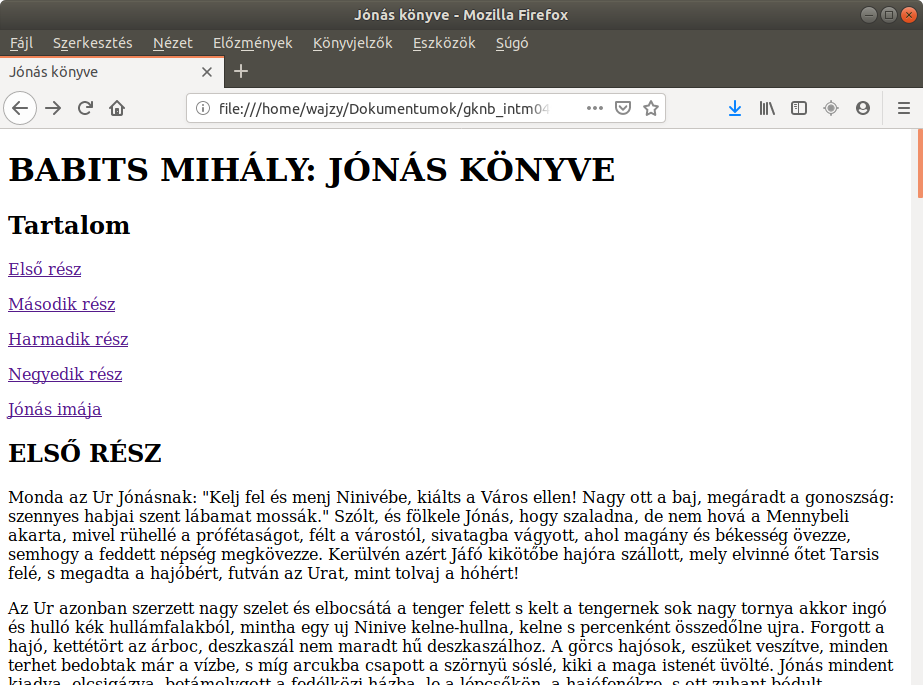
\includegraphics[scale=.15]{jonas.png}
        \end{exampleblock}
      \end{center}
  \end{columns}
\end{frame}

%36
\begin{frame}
  Kép egyes részei kijelölhetők, és más-más oldalakra hivatkozhatnak.
  \begin{enumerate}
    \item Megjeleníteni a képet \texttt{<img>} elemmel, elhelyezni benne a \texttt{usemap} attribútumot, melynek értéke \#-tel kezdődik, és a \emph{térkép} nevével folytatódik.
    \item Létrehozni valahol egy \texttt{<map>} elemet, melynek \texttt{name} attribútuma tartalmazza a térkép nevét.
    \item Ebbe beágyazni \texttt{<area>} üres elemeket, melynek \texttt{shape} attribútuma egy alakzatot, \texttt{coords} attribútuma pedig ennek koordinátáit definiálja:
    \begin{itemize}
      \item \texttt{rect} téglalap, két átellenes sarok X, Y koordinátájával
      \item \texttt{circle} kör, középpont X, Y koordinátája, sugár
      \item \texttt{poly} poligon, egymást követő pontok x, Y koordinátái; az utolsót összeköti az elsővel
      \item \texttt{default} a teljes kép külön nem jelölt része
    \end{itemize}
    \item Az \texttt{<area>} \texttt{href} attribútuma definiálja a célt.
  \end{enumerate}
\end{frame}

%37
\begin{frame}
  A \textattachfile{cyclist.jpg}{cyclist.jpg} felhasználásával hozza létre a \textattachfile{terkepek.html}{terkepek.html} weboldalt! A képen kijelölendő területek alakja, koordinátái és célja az alábbi:
  
    \begin{table}
      \resizebox{\textwidth}{!}{
      \begin{tabular}{llp{3cm}l}
      Mit jelöl ki? & Alakzat  & Koordináták                                                                                     & Cél                                                            \\ \hline
      Első kereket  & Kör      & 217, 813, 145                                                                                     & https://ebike.hu/termekek/kerek/felni/                         \\
      Kosarat       & Téglalap & 102, 420, 256, 643                                                                                 & https://ebike.hu/termekek/kiegeszitok/csomagtarto/elore/       \\
      Gyerekülést   & Poligon  & 895, 346, 859, 409, 841, 480, 774, 507, 744, 579, 771, 690, 742, 732, 832, 724, 813, 606, 873, 589, 873, 466, 915, 358 & https://ebike.hu/termekek/kiegeszitok/gyermekules/hatra-vazra/ \\
      Maradék részt & ~        & ~                                                                                               & https://ebike.hu/                                              \\
      \end{tabular}
      }
    \end{table}
\end{frame}

%38
\begin{frame}
  Szerver oldali térképek\\
  A kattintás helyét küldi a szervernek URL-be kódolva.
  \begin{enumerate}
    \item Hozzunk létre hivatkozást a webhelyre! (\texttt{<a>} elem)
    \item Ágyazzuk bele a képet (\texttt{<img>}) az \texttt{ismap} attribútummal!
  \end{enumerate}
  Például: \texttt{<a href="weblap.html"><img alt="Kép" src="kep.jpeg" ismap="ismap"></a>}
  \vfill
  Feladat: alakítsa át az előző feladatot szerver oldali térképet használóra! (\textattachfile{terkepSzerver.html}{Megoldás})
\end{frame}


\subsection{Táblázatok}

%39
\begin{frame}
  Táblázatok kötelező elemei:
  \begin{description}[m]
    \item[\texttt{<table>}] \hfill \\ Maga a táblázat.
    \item[\texttt{<tr>}] (table row) \hfill \\ A táblázat egy sora, a \texttt{<table>} elembe kell beágyazni.
    \item[\texttt{<td>}] (table data) \hfill \\ A sor egy cellája, a \texttt{<tr>} elembe kell beágyazni, vagy
    \item[\texttt{<th>}] (table header) \hfill \\ fejléc cella. (Általában alapértelmezés szerint félkövér, középre zárt megjelnítésű.)
  \end{description}
\end{frame}


\subsection{Listák, felsorolások}

\subsection{Listák, felsorolások}

%49
\begin{frame}
  Háromféle felsorolás (lista) létezik a HTML-ben:
  \begin{enumerate}
    \item Számozatlan
    \item Számozott
    \item Definíciós
  \end{enumerate}
  \vfill
  Rendkívül rugalmasan formázható CSS-ből, pl. \hiv{\href{https://www.christianpinder.com/articles/menu-using-html-lists-and-css/}{weboldalak menürendszere}} is kialakítható
\end{frame}

%50
\begin{frame}
  \begin{itemize}
    \item Számozatlan felsorolás: \texttt{<ul>} (unordered list) elemmel
    \item Ennek elemei: beágyazott \texttt{<li>} (list item) elemekkel
  \end{itemize}
  \begin{columns}[T]
    \column{0.6\textwidth}
      \begin{exampleblock}{\textattachfile{bevasarlas.html}{bevasarlas.html}}
        \footnotesize
        \lstinputlisting[style=HTML,linerange={8-13},numbers=left,firstnumber=8]{bevasarlas.html}
      \end{exampleblock}
    \column{0.35\textwidth}
      \centering 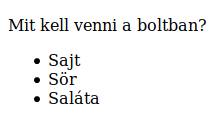
\includegraphics[width=\textwidth]{bevasarlas.png}
  \end{columns}
\end{frame}

%51
\begin{frame}
  \begin{columns}[c]
    \column{0.5\textwidth}
      Feladat: készítsen a mellékelt ábrának megfelelően egy számozatlan felsorolást tartalmazó weblapot! (Forrás: \hiv{\href{https://www.buvosszakacs.com/2014/04/13/diy-sor-bevalt-receptek/}{Bűvös Szakács}})
    \column{0.5\textwidth}
      \begin{exampleblock}{\textattachfile{sor.html}{sor.html}}
        \centering 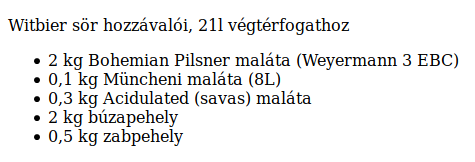
\includegraphics[width=\textwidth]{sor.png}
      \end{exampleblock}
  \end{columns}
\end{frame}

%52
\begin{frame}
  \begin{itemize}
    \item Számozott felsorolás: \texttt{<ol>} (ordered list) elemmel, attribútumai:
    \begin{description}[m]
      \item[\texttt{type}] felsorolásjel típusa \hfill \\ 
        \begin{table}[]
        \begin{tabular}{ll}
        \textbf{Att. érték} & \textbf{Felsorolásjel}       \\\hline
        1                   & Arab számok (alapértelmezés) \\
        A                   & Latin nagybetűk              \\
        a                   & Latin kisbetűk               \\
        I                   & Nagybetűs római számok       \\
        i                   & Kisbetűs római számok       
        \end{tabular}
        \end{table}
      \item[\texttt{start}] \hfill \\ Az első elem sorszáma
      \item[\texttt{reversed}] \hfill \\ Csökkenő sorrendet ír elő
    \end{description}
    \item Ennek elemei: beágyazott \texttt{<li>} (list item) elemekkel
  \end{itemize}
\end{frame}

%53
\begin{frame}
  \begin{columns}[c]
    \column{0.5\textwidth}
      \begin{exampleblock}{\textattachfile{futurama.html}{futurama.html} (\kiemelN{\href{https://www.reddit.com/r/futurama/comments/4ds4vf/what_is_this_in_reference_to/}{Futurama}})}
        \lstinputlisting[style=HTML,linerange={8-12},numbers=left,firstnumber=8]{futurama.html}
      \end{exampleblock}
    \column{0.45\textwidth}
      \begin{center}
        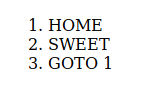
\includegraphics[width=.8\textwidth]{futurama.png}
        \vfill
        
\includegraphics[width=.8\textwidth]{futurama_orig.png}
      \end{center}
  \end{columns}
\end{frame}

%54
\begin{frame}
  \begin{columns}[c]
    \column{0.5\textwidth}
      Kiindulva a \textattachfile{jaegermeister.txt}{jaegermeister.txt} fájlból, hozza létre az ábrán látható HTML fájlt!
    \column{0.45\textwidth}
      \begin{exampleblock}{\textattachfile{jaegermeister.html}{jaegermeister.html}}
        \centering 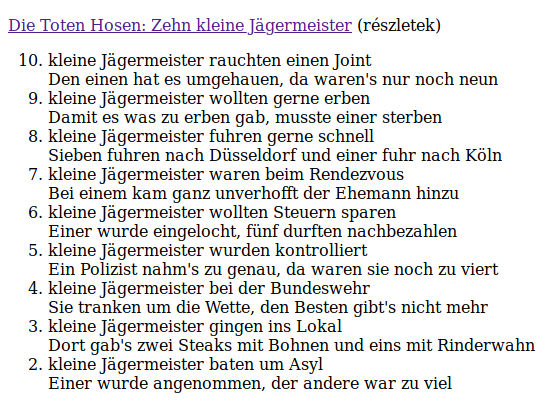
\includegraphics[width=\textwidth]{jaegermeister.png}
      \end{exampleblock}
  \end{columns}
\end{frame}

%55
\begin{frame}
  \begin{columns}[T]
    \column{0.45\textwidth}
      Többszintű felsorolások
      \begin{itemize}
        \item \texttt{<li>} elem belsejébe újabb felsorolás ágyazható
        \item A számozás újrakezdődik az első szinten $\to$ \hiv{\href{https://stackoverflow.com/questions/10405945/html-ordered-list-1-1-1-2-nested-counters-and-scope-not-working}{CSS}}
      \end{itemize}
      \vfill
      \centering 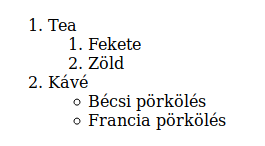
\includegraphics[width=\textwidth]{tobbszintu.png}
    \column{0.5\textwidth}
      \begin{exampleblock}{\textattachfile{tobbszintu.html}{tobbszintu.html}}
        \scriptsize
        \lstinputlisting[style=HTML,linerange={8-21},numbers=right,firstnumber=8]{tobbszintu.html}
      \end{exampleblock}
  \end{columns}
\end{frame}

%56
\begin{frame}
  \begin{itemize}
    \item Definíciós lista létrehozása \texttt{<dl>} (description list) elemmel
    \item A kifejezés megadása \texttt{<dl>}-be ágyazott \texttt{<dt>} (term) elemmel
    \item Magyarázat az ezt követő \texttt{<dd>} (description) elemben
  \end{itemize}
  \begin{columns}[T]
    \column{0.6\textwidth}
      \begin{exampleblock}{\textattachfile{froccs.html}{froccs.html}}
        \scriptsize
        \lstinputlisting[style=HTML,linerange={8-15},numbers=left,firstnumber=8]{froccs.html}
      \end{exampleblock}
    \column{0.35\textwidth}
      \centering 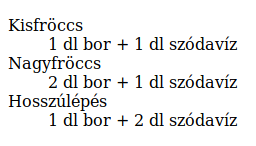
\includegraphics[width=\textwidth]{froccs.png}
  \end{columns}
\end{frame}

%57
\begin{frame}
   Hozza létre az ábrán látható HTML fájlt!
  \begin{exampleblock}{\textattachfile{betuszavak.html}{betuszavak.html}}
    \centering 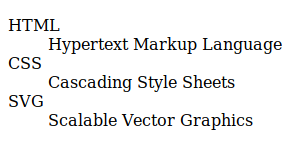
\includegraphics[scale=0.5]{betuszavak.png}
  \end{exampleblock}
\end{frame}


\subsection{Soron belüli keretek}

%58
\begin{frame}
  Egy HTML oldal megjelenítése egy másik oldalban: \texttt{<iframe>} elemmel
  \vfill
  Attribútumok:
  \begin{description}[m]
    \item[\texttt{src}] (source) \hfill \\ A keretbe betöltendő dokumentum URL-je
    \item[\texttt{width}] \hfill \\ Keret szélessége képpontban
    \item[\texttt{height}] \hfill \\ A keret magassága képpontban
  \end{description}
\end{frame}

%59
\begin{frame}
  További attribútumok:
  \begin{description}[m]
    \item[\texttt{name}] \hfill \\ Ez azonosítja a keretet, amibe pl. új tartalom tölthető egy \texttt{<a>} elemmel, ha annak \texttt{target} attribútuma a \texttt{name} értékét tartalmazza
    \item[\texttt{srcdoc}] \hfill \\ Megjelenítendő dokumentum HTML kódja (magasabb prioritású, mint \texttt{src}, ha támogatott)
    \item[\texttt{sandbox}] \hfill \\ Megjelenítési környezet korlátozásainak feloldása (\texttt{allow-forms}, \texttt{allow-pointer-lock}, \texttt{allow-popups}, \texttt{allow-same-origin}, \texttt{allow-scripts}, \texttt{allow-top-navigation}) \hiv{\href{https://www.html5rocks.com/en/tutorials/security/sandboxed-iframes/}{részletek}}
  \end{description}
\end{frame}

%60
\begin{frame}
  Megjegyzések
  \begin{itemize}
    \item Az \texttt{srcdoc}-ot csak az \hiv{\href{https://caniuse.com/\#search=iframe\%20srcdoc}{újabb}} böngészők támogatják
    \item A webszerverek az \hiv{\href{https://developer.mozilla.org/hu/docs/Web/HTTP/Headers/X-Frame-Options}{X-Frame-Options}} HTTP válasz fejléccel kérhetik az ezt támogató böngészőktől, hogy ne engedjék a lapot \texttt{<iframe>}-be tölteni.
    \item \texttt{src}+\texttt{sandbox} biztonságos korszerű böngészőkben, de \kiemel{nem biztonságos a \texttt{sandbox}-ot nem támogatókban!}
    \item \texttt{srcdoc}+\texttt{sandbox} biztonságos korszerű böngészőkben, és nem működik (=biztonságos) az elavultakban
  \end{itemize}
\end{frame}

%61
\begin{frame}
  \begin{columns}[c]
    \column{0.6\textwidth}
      \begin{exampleblock}{\textattachfile{iframe.html}{iframe.html}}
        \footnotesize
        \lstinputlisting[style=HTML,linerange={8-14},numbers=left,firstnumber=8]{iframe.html}
      \end{exampleblock}
    \column{0.35\textwidth}
      \centering 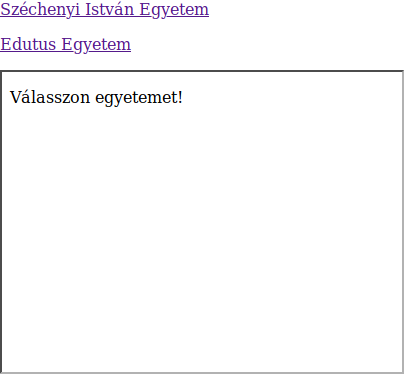
\includegraphics[width=\textwidth]{iframe.png}
  \end{columns}
\end{frame}


\subsection{A fejrész elemei}

\subsection{A fejrész elemei}

%62
\begin{frame}
  A \texttt{<head>} tartalmazza a HTML oldal metaadatait. HTML5-től elhagyható, de javasolt használni. Beágyazható elemek:
  \begin{description}[m]
    \item[\texttt{<title>}] \hfill \\ A dokumentum címe, kötelező.
    \item[\texttt{<style>}] \hfill \\ CSS stílusok, formázás megadása; ált. jobb külön fájlba helyezni, ld. később 
    \item[\texttt{<base>}] \hfill \\ A relatív URL-ek a \texttt{href} értéke alapján lesznek értelmezve. A \texttt{target} más elemek \texttt{target} attribútumának alapértelmezett értékét adja meg.
  \end{description}
\end{frame}

%63
\begin{frame}
  \begin{description}[m]
    \item[\texttt{<link>}] \hfill \\ Külső erőforrás és a dokumentum kapcsolatát adja meg. Jellemző alkalmazásai:
    \begin{itemize}
      \item Stíluslap meghatározása: \texttt{href}-ben a CSS fájl URL-je, \texttt{rel} (relationship) \emph{stylesheet}, a \texttt{type} \emph{text/css} értékű.
      \item Ikon (favicon = favorite icon) beállítás: \texttt{href}-ben az ikon URL-je, \texttt{rel} \emph{icon}, a \texttt{type} pl. \emph{image/svg+xml} értékű. (További \hiv{\href{https://en.wikipedia.org/wiki/Favicon}{részletek}}.)
    \end{itemize}
    \item[\texttt{<meta>}] \hfill \\ HTTP fejlécek kulcs (\texttt{http-equiv} attribútum) - érték (\texttt{content} attribútum) párok formájában történő megadására. Jellemző kulcsok:
    \begin{itemize}
      \item \emph{content-type}, a MIME típus és karakterkódolás megadására: \texttt{content="text/html; charset=UTF-8"} $\to$ HTML5-től: csak a \texttt{charset="UTF-8"} attribútummal
      \item \emph{refresh}, automatikus újratöltés, pl. percenként: \texttt{content="60"}
    \end{itemize}
  \end{description}
\end{frame}

%64
\begin{frame}
  \begin{description}[m]
    \item[\texttt{<meta>}] \hfill \\ Metaadatok kulcs (\texttt{name} attribútum) - érték (\texttt{content} attribútum) párok formájában történő megadására. Jellemző kulcsok:
    \begin{itemize}
      \item \emph{description}, weboldal általános leírása
      \item \emph{keywords}, kulcsszavak keresőmotoroknak az oldal tartalmához kapcsolódóan
      \item \emph{author}, szerző
      \item \emph{viewport}, nézetablak beállítás, \texttt{content="width=device-width, initial-scale=1.0"}. Probléma: mobil eszközök nagy felbontásúak, de kis méretűek, számítógép-kijelzőre optimalizált oldalak gyenge felhasználói élménnyel használhatók. \emph{width=device-width}: a nézetablak szélessége alkalmazkodik az eszköz szélességéhez. \emph{initial-scale=1.0} nagyítás kezdeti értéke. \hiv{\href{https://www.quirksmode.org/mobile/viewports2.html}{Részletek}}
    \end{itemize}
  \end{description}
\end{frame}

%65
\begin{frame}
  \begin{description}[m]
    \item[\texttt{<script>}] \hfill \\ JavaScript programok megadására; előnyösebb a \texttt{<body>} végébe tenni (DOM felépül, az oldalbetöltést a JS kód nem lassítja).
    \item[\texttt{<noscript>}] \hfill \\ JavaScript támogatás hiányában a közrezárt szöveget megjeleníti. HTML5-től a \texttt{body}-ba is kerülhet.
  \end{description}
  \vfill
  HTML5-től a \texttt{<html>}, \texttt{<head>} és \texttt{<body>} elemek elhagyhatók, de ezt nem ajánljuk.
\end{frame}

%66
\begin{frame}
  \begin{exampleblock}{\textattachfile{fejresz.html}{fejresz.html} (\textattachfile{fejresz/fejresz.css}{fejresz/fejresz.css}, \textattachfile{fejresz/fejresz.js}{fejresz/fejresz.js}, \textattachfile{fejresz/fejresz2.html}{fejresz/fejresz2.html})}
    \scriptsize
    \lstinputlisting[style=HTML,linerange={3-16},numbers=left,firstnumber=3]{fejresz.html}
  \end{exampleblock}
\end{frame}

%66
\begin{frame}
  \begin{exampleblock}{\textattachfile{fejresz.html}{fejresz.html}}
    \lstinputlisting[style=HTML,linerange={17-22},numbers=left,firstnumber=17]{fejresz.html}
  \end{exampleblock}
  \begin{columns}[T]
    \column{0.3\textwidth}
      \centering 
\includegraphics[width=\textwidth]{fejresz_vilagos.png}
    \column{0.3\textwidth}
      \centering 
\includegraphics[width=\textwidth]{fejresz_sotet.png}
  \end{columns} 
\end{frame}

%67
\begin{frame}
  A \textattachfile{macska.txt}{macska.txt} fájlból kiindulva készítse el a \textattachfile{macska.html}{macska.html} oldalt az ábrának megfelelően!
  \begin{columns}[c]
    \column{0.65\textwidth}
      \begin{enumerate}
        \item Az oldal címe legyen \emph{Macska}!
        \item Az oldalt formázza meg a \textattachfile{macska.css}{macska.css} stíluslap segítségével!
        \item Jelenítse meg a \textattachfile[mimetype=image/png]{macska.png}{macska.png} fájlt ikonként (favicon)!
        \item A dokumentum kódolása UTF-8 szerint történjen!
        \item Készítsen \emph{ismertetőt}, adjon meg \emph{kulcsszavakat} a keresőmotorok számára! Adja meg a saját nevét \emph{szerzőként}!
        \item A nézetablak szélességét igazítsa a megjelenítő szélességéhez, a nagyítás legyen 1x-es!
        \item Szúrja be a macska képét (\textattachfile[mimetype=image/jpeg]{macska.jpeg}{macska.jpeg})!
      \end{enumerate}      
    \column{0.3\textwidth}
      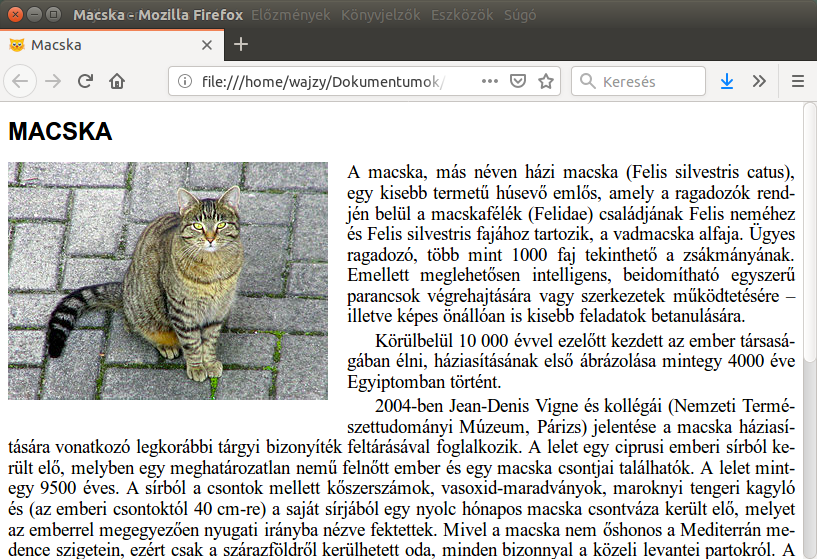
\includegraphics[width=\textwidth]{macska_screenshot.png}
  \end{columns} 
\end{frame}


\subsection{Oldalak főbb részeinek jelölése}

\subsection{Oldalak főbb részeinek jelölése}

%68
\begin{frame}
  A HTML szemantikus elemei az oldal funkcionális részeinek jelölésére:
  \begin{description}[m]
    \item[\texttt{<main>}] \hfill \\ A dokumentum legfőbb tartalmát jelöli, ami nem ismétlődik más oldalakon, azaz nem tartalmazza pl. a menüsort, oldal logot, szerzői jogi információt. \kiemel{Csak egyszer fordulhat elő} a dokumentumban! Nem lehet az \texttt{<article>}, \texttt{<aside>}, \texttt{<footer>}, \texttt{<header>}, \texttt{<nav>} leszármazottja. Célja: akadálymentesítés, Safari olvasó funkciója is ezt emeli ki.
    \item[\texttt{<nav>}] \hfill \\ Az oldal legfontosabb navigációs hivatkozásainak gyűjteménye, pl. menü, tartalomjegyzék. A menüt gyakran CSS formázott \texttt{<ul>} elemekkel valósítják meg. Több \texttt{<nav>} is lehet egy oldalon, pl. külön az oldalon belüli, és azon kívülre mutató hivatkozásoknak.
  \end{description} 
\end{frame}

%69
\begin{frame}
  \begin{description}[m]
    \item[\texttt{<article>}] \hfill \\ Az oldal többi részétől függetlenül, önmagában is értelmes tartalmi rész, pl. fórum- vagy blogbejegyzés, hír. Jellemzően címsorral kezdődik. Egy oldalon belül többször is előfordulhat, akár egymásba is ágyazhatók (pl. blogbejegyzés és az arra adott reakciók). A megjelenés dátumát gyakran tartalmazza beágyazott \texttt{<time>} elemmel (a \texttt{datetime} attribútummal gépek is felismerik).
    \item[\texttt{<section>}] \hfill \\ Dokumentum egy része, fejezete, de akár fejléce, lábléce is lehet. Ajánlott címsorral ellátni. Nem lehet az \texttt{<address>} leszármazottja.
  \end{description} 
\end{frame}

%70
\begin{frame}
  \begin{description}[m]
    \item[\texttt{<aside>}] \hfill \\ A tartalomhoz lazán kapcsolódó kiegészítés, megjegyzés. Akadálymentesítési okokból használják a \texttt{role} attribútumot.
    \item[\texttt{<header>}] \hfill \\ Általában a dokumentum bevezetőjét, navigációs hivatkozásokat tárol. Gyakran tartalmaz címsor (\texttt{<h1>}-\texttt{<h6>}) elemeket, logot, szerzőt. Többször is előfordulhat a dokumentumban, pl. több \texttt{<article>} elejében.
    \item[\texttt{<footer>}] \hfill \\ Egy dokumentum vagy fejezet lábléce. Jellemzően a szerző nevét, szerzői jogi információt, kapcsolatfelvétel módját (ld. \texttt{<address>}), oldaltérképet, impresszumot, stb. tartalmaz. Többször is előfordulhat egy dokumentumban (pl. minden \texttt{<article>} végén).
  \end{description} 
\end{frame}

%71
\begin{frame}
  \begin{exampleblock}{\textattachfile{reszek.html}{reszek.html}}
    \footnotesize
    \lstinputlisting[style=HTML,linerange={7-19},numbers=left,firstnumber=7]{reszek.html}
  \end{exampleblock}
\end{frame}

%72
\begin{frame}
  \begin{exampleblock}{\textattachfile{reszek.html}{reszek.html}}
    \footnotesize
    \lstinputlisting[style=HTML,linerange={20-26},numbers=left,firstnumber=20]{reszek.html}
    \lstinputlisting[style=HTML,linerange={34-37},numbers=left,firstnumber=34]{reszek.html}
  \end{exampleblock}
\end{frame}

%73
\begin{frame}
  \begin{exampleblock}{\textattachfile{reszek.html}{reszek.html}}
    \footnotesize
    \lstinputlisting[style=HTML,linerange={47-56},numbers=left,firstnumber=47]{reszek.html}
  \end{exampleblock}
\end{frame}

%74
\begin{frame}
  \begin{exampleblock}{\textattachfile{reszek.html}{reszek.html}}
    \footnotesize
    \lstinputlisting[style=HTML,linerange={103-115},numbers=left,firstnumber=103]{reszek.html}
  \end{exampleblock}
\end{frame}

%75
\begin{frame}
  Tartalom megjelenítése / elrejtése
  \begin{columns}[T]
    \column{0.67\textwidth}
      \begin{description}[m]
        \item[\texttt{<details>}] \hfill \\ Interaktív oldalrész, amit a felhasználó elrejthet/megjeleníthet (alapértelmezetten rejtett; megjeleníthető az \texttt{open} attribútummal). Gyakorlatilag bármi beleágyazható.
        \item[\texttt{<summary>}] \hfill \\ A blokk kattintható fejléce, mindig látszik.
      \end{description}
    \column{0.3\textwidth}
      \begin{exampleblock}{\textattachfile{reszletek.html}{reszletek.html}}
        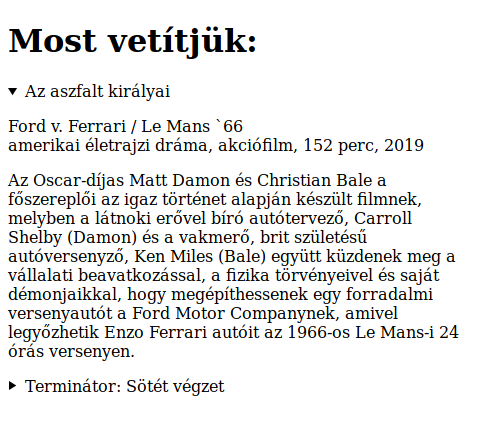
\includegraphics[width=\textwidth]{reszletek.png}
      \end{exampleblock}
  \end{columns}
\end{frame}

%76
\begin{frame}
  \begin{exampleblock}{\textattachfile{reszletek.html}{reszletek.html}}
    \footnotesize
    \lstinputlisting[style=HTML,linerange={9-14},numbers=left,firstnumber=9]{reszletek.html}
    \lstinputlisting[style=HTML,linerange={20-21},numbers=left,firstnumber=20]{reszletek.html}
  \end{exampleblock}
\end{frame}

%77
\begin{frame}
  A \textattachfile{c64.txt}{c64.txt} fájl felhasználásával készítse el a \texttt{c64.html} fájlt!
  \begin{itemize}
    \item Az újság neve és a rovatok kerüljenek a dokumentum fejlécébe!
    \item Készítsen navigációs sávot az \emph{index}, \emph{c64.com} és \emph{Wikipédia} elemekből!
    \item Az oldal \emph{fő} része tartalmazza a teljes cikket!
    \item A cikknek is legyen fejléce, ami a \emph{cikk címéből}, \emph{szerzőjéből} és a \emph{megjelenés idejéből} áll!
    \item Az \emph{,,Egy maroknyi dollárért''} és a \emph{,,Specifikáció''} legyen a cikk két fejezetének címe!
    \item A \emph{,,Microprocesszor''} és \emph{,,Video hardver...''} kattintásra jelenjen meg/tűnjön el!
    \item Az \emph{,,Önök írták''} legyen az ,,oldalsáv'' fejléce!
  \end{itemize}
\end{frame}

%78
\begin{frame}
  \begin{exampleblock}{\textattachfile{c64.html}{c64.html}}
    \centering 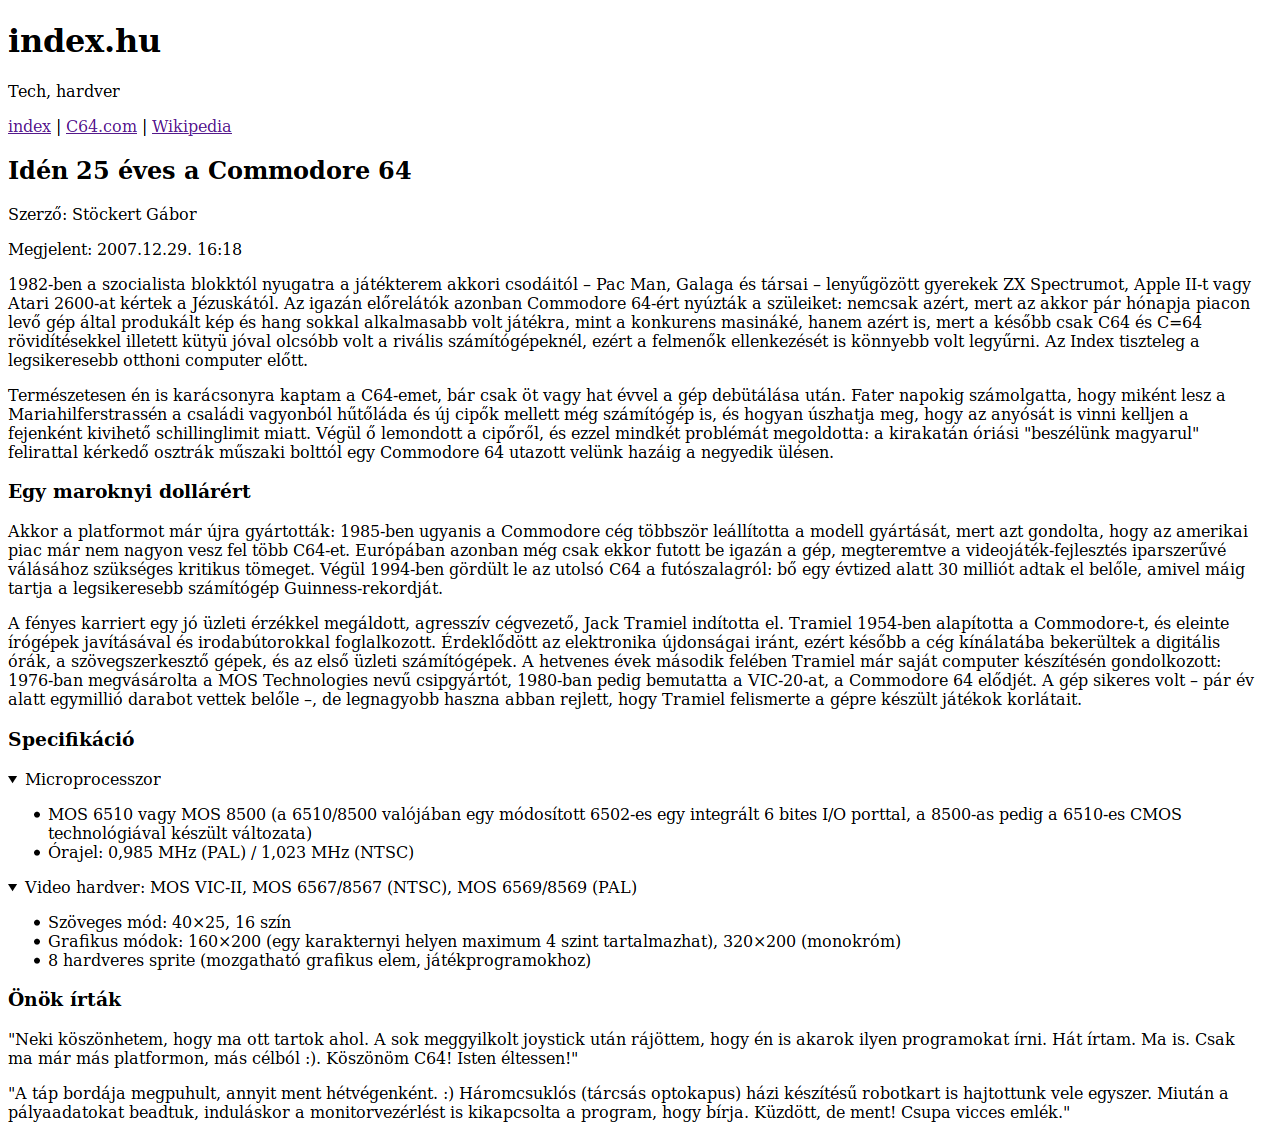
\includegraphics[scale=.14,]{c64.png}
  \end{exampleblock}
\end{frame}


% blokkszintű és soron belüli elemek összefoglalója
% class és id attribútumok
% Data URI

\end{document}
